\documentclass[a4paper]{article}
\usepackage[utf8]{inputenc}


%=-=-=-=-=-=-=-=-=-=-=-=-=-=-=-=-=-=-=-=-=-=-=-=-=-=-=-=-=-=-=-=-=-=-=-=-=-=-=-=-
% PREAMBLE
%=-=-=-=-=-=-=-=-=-=-=-=-=-=-=-=-=-=-=-=-=-=-=-=-=-=-=-=-=-=-=-=-=-=-=-=-=-=-=-=-

%%%%%%%%%%%%%%%%%%%%%%%%%%%%%%%%%%%%%%%%%%%%%%%%%%%%%%%%%%%%%%%%%%%%%
% Important styling notes
%%
% For now, to include img.jpg in img/path/to/img.jpg, just use:
% path/to/img.jpg - for details see style.tex
%=-=-=-=-=-=-=-=-=-=-=-=-=-=-=-=-=-=-=-=-=-=-=-=-=-=-=-=-=-=-=-=-=-=-=-=-=-=-=-=-
% Packages
%%
%\usepackage{fullpage} % Package to use full page
\usepackage[top=1in,bottom=1in,left=1in,right=1in,heightrounded]{geometry}

\usepackage{parskip}                    % Package to tweak paragraph skipping
\usepackage{amsmath}                    % standard
\usepackage{amssymb}                    % standard - Double R symbol etc.
\usepackage{hyperref}
\usepackage{amsthm}                     % standard - theorem, definition, etc.
\usepackage{multicol}                   % multiple columns for numbering
\usepackage{enumitem}                   % standard - enumerate styles
\usepackage[utf8]{inputenc}
\usepackage{scrextend}                  % indentation
\usepackage{graphicx}                   % standard - add figures
\usepackage{float}                      % standard - figure position, use [H] option
\usepackage{pifont}                     % symbols http://willbenton.com/wb-images/pifont.pdf
                                        % e.g. \ding{51}
\usepackage{gensymb}                    % degree symbol \degree
\usepackage{xcolor}                     % bg color
\hypersetup{
    colorlinks,
    linkcolor={black!50!black},
    citecolor={blue!50!black},
    urlcolor={blue!80!black}
}
\usepackage{framed}                     % bg color
\usepackage[T1]{fontenc}                % small caps
\usepackage{sectsty}                    % headings colour
\usepackage{mathtools}                  % Loads amsmath
\usepackage{amsthm,thmtools,xcolor}     % coloured theorem
\usepackage[toc,page]{appendix}         % reference to appendix
%\usepackage{titlesec}                   % change chapter, section, etc. formats
\usepackage{xifthen}                    % if, else
\usepackage{etoolbox}
% format numbering in theorem, lemma, etc. environment
\AtBeginEnvironment{theorem}{\setlist[enumerate, 1]{font=\upshape,  wide=0.5em, before=\leavevmode}}
\AtBeginEnvironment{lemma}{\setlist[enumerate, 1]{font=\upshape,  wide=0.5em, before=\leavevmode}}
\usepackage[letterspace=150]{microtype} % \textls{<letterspaced text>} % 0 <= letterspace <= 1000, 1000 = M space
\usepackage{letltxmacro}                % renew commands?
\usepackage{minted}                     % package to list code
    % otherwise minted goes off the page
    \setmintedinline{breaklines}
\usepackage{subfig}
\usepackage{eso-pic}                    % title page bg pic
\usepackage{varwidth}
\PassOptionsToPackage{svgnames}{xcolor}
\usepackage{fontawesome}                % \faQuestionCircle
\usepackage{marvosym}                   %\Pointinghand
\usepackage{mdframed}                   % easy outline frames
\usepackage[many]{tcolorbox}            % colour box for theorem styles
\usepackage{array,booktabs,calc} % table figs and text
\usepackage{comment}                    % \begin{comment}
\usepackage{fancyhdr}                   % page headings
\usepackage{mdframed}                   % boxes
\usepackage[backend=biber,sorting=none,style=ieee]{biblatex}
\usepackage{caption}
%%% caption options {
%\DeclareCaptionFont{white}{\color{white}}
\DeclareCaptionFormat{listing}{\colorbox{magenta!30!gray}{\parbox{\textwidth}{#1#2#3}}}
\captionsetup[lstlisting]{format=listing,labelfont={bf,small},textfont=small,skip=-1pt}
%%% }
\addbibresource{bibliography.bib}
\usepackage{url}
\usepackage{textcomp}
\usepackage[makeroom]{cancel}           % crossed symbols - \cancel{}, \bcancel{}, xcancel{}
\usepackage{algorithm}
\usepackage[noend]{algpseudocode}
\usepackage{tikz}
\usetikzlibrary{arrows.meta,positioning,quotes} % arrows and nodes in tikz
\usepackage{marginnote}                 % things in page margin by \marginnote{...}
\usepackage{pgfplots}
\usepackage{pstricks-add,pst-slpe}      % for fancy tikz arrows
%\usepackage{titlesec}                  % title style
\usepackage{lmodern}                    % a font
\usepackage{titletoc}                   % Required for manipulating the table of contents
\usepackage{titlesec}                   % Allows customization of titles
\usepackage{fouriernc}                  % Use the New Century Schoolbook font
\usepackage{booktabs}                   % better tables
\usepackage{stmaryrd }                  % \varoast
\usepackage{listings}                   % code listings
\usepackage{longtable}                  % table across multiple pages
\usepackage{todonotes}                  % TODO bubbles by \todo{...} command
\usepackage{changepage}                 % paragraph margins
\usepackage{tikz}
\usetikzlibrary{calc}
\usepackage{eso-pic}
\usepackage{transparent}



%=-=-=-=-=-=-=-=-=-=-=-=-=-=-=-=-=-=-=-=-=-=-=-=-=-=-=-=-=-=-=-=-=-=-=-=-=-=-=-=-
% Colours for various things
%%


\definecolor{shadecolor}{rgb}{1.,0.933,0.96} % bg color, r,g,b <= 1
\definecolor{medium_blue}{RGB}{60,125,190}
\definecolor{dark_blue}{RGB}{25,60,85}
\definecolor{dark_red}{RGB}{77,16,16}
\definecolor{LightPink}{rgb}{0.92.,0.8,0.84} % bg color, r,g,b <= 1
\definecolor{LighterPink}{rgb}{1.,0.94,0.97} % bg color, r,g,b <= 1
\definecolor{LightestPink}{rgb}{1.,0.95,0.99} % bg color, r,g,b <= 1
\definecolor{DarkestPink}{rgb}{0.36, 0.0, 0.18}
\definecolor{DarkerPink}{rgb}{0.41, 0.0, 0.21}
\definecolor{DarkPink}{rgb}{0.55, 0.05, 0.37}
\definecolor{lightestestpink}{RGB}{255,248,252}
\definecolor{codegray}{rgb}{0.5,0.5,0.5}
\definecolor{codegrayblue}{rgb}{0.35,0.35,0.47}



%=-=-=-=-=-=-=-=-=-=-=-=-=-=-=-=-=-=-=-=-=-=-=-=-=-=-=-=-=-=-=-=-=-=-=-=-=-=-=-=-
% Define my own theorem styles
%%

% "base" styles
\declaretheoremstyle[
  headfont=\color{DarkPink}\bfseries,
  bodyfont=\itshape,
]{colored}

\declaretheoremstyle[
  headfont=\color{DarkPink}\bfseries,
  bodyfont=\normalfont,
]{colored_upright}

% theorems (corollaries, etc) themselves, inherit from my style above
% Usage:
% \begin{theorem} \end{theorem}, \begin{lemma} \end{lemma}, ...
\declaretheorem[
	numberwithin=section,
 	style=colored,
	name=\textsc{Theorem},
]{theorem}

\tcolorboxenvironment{theorem}{
  boxrule=0pt,
  boxsep=2pt,
  colback={magenta!25!white},
  colframe=DarkPink,
  enhanced jigsaw, 
  borderline west={2pt}{0pt}{DarkPink},
  sharp corners,
  before skip=5pt,
  after skip=5pt,
  breakable,
  right=0mm % for equations
}

\declaretheorem[
	numberwithin=section,
 	style=colored,
	name=\textsc{Corollary},
]{corollary}

\tcolorboxenvironment{corollary}{
  boxrule=0pt,
  boxsep=1pt,
  colback={magenta!10!white},
  colframe=DarkPink,
  enhanced jigsaw, 
  borderline west={2pt}{0pt}{DarkPink},
  sharp corners,
  before skip=5pt,
  after skip=5pt,
  breakable,
  right=0mm % for equations
}

\declaretheorem[
	numberwithin=section,
	style=colored,
	name=\textsc{Lemma},
]{lemma}

\tcolorboxenvironment{lemma}{
  boxrule=0pt,
  boxsep=1pt,
  colback={magenta!10!white},
  colframe=DarkPink,
  enhanced jigsaw, 
  borderline west={2pt}{0pt}{DarkPink},
  sharp corners,
  before skip=5pt,
  after skip=5pt,
  breakable,
  right=0mm % for equations
}

\declaretheorem[
	numberwithin=section,
	style=colored,
	name=\textsc{Definition},
]{definition}

\tcolorboxenvironment{definition}{
  boxrule=0pt,
  boxsep=1pt,
  colback={magenta!25!white},
  colframe=DarkPink,
  enhanced jigsaw, 
  borderline west={2pt}{0pt}{DarkPink},
  sharp corners,
  before skip=5pt,
  after skip=5pt,
  breakable,
  right=0mm % for equations
}

\declaretheorem[
	numberwithin=section,
  	style=colored,
  	name=\textsc{Example},
]{exmp}

\declaretheorem[
	numberwithin=section,
  	style=colored,
  	name=\textsc{Solution},
]{soln}

%%% code listings
\lstdefinestyle{code1}{
    backgroundcolor=\color{lightestestpink},   
    commentstyle=\color{codegrayblue},
    keywordstyle=\color{DarkerPink},
    numberstyle=\tiny\color{codegray},
    stringstyle=\color{black!40!cyan},
    basicstyle=\small\ttfamily,
    breakatwhitespace=false,
    breaklines=true,        
    captionpos=t,             
    keepspaces=true,        
    numbers=left,           
    numbersep=5pt,
    showspaces=false, 
    showstringspaces=false,
    showtabs=false,
    tabsize=4
}

%%% code listings
\lstdefinestyle{code1}{
    backgroundcolor=\color{lightestestpink},   
    commentstyle=\color{codegrayblue},
    keywordstyle=\color{DarkerPink},
    numberstyle=\tiny\color{codegray},
    stringstyle=\color{black!40!cyan},
    basicstyle=\small\ttfamily,
    breakatwhitespace=false,
    breaklines=true,        
    captionpos=t,             
    keepspaces=true,        
    numbers=left,           
    numbersep=5pt,
    showspaces=false, 
    showstringspaces=false,
    showtabs=false,
    tabsize=4
}


\lstdefinestyle{terminal}{
    backgroundcolor=\color{black!5},   
    commentstyle=\color{codegrayblue},
    keywordstyle=\color{DarkerPink},
    %numberstyle=\tiny\color{codegray},
    stringstyle=\color{black!40!cyan},
    basicstyle=\small\ttfamily,
    numbers=none,
    breakatwhitespace=false,
    breaklines=true,        
    %captionpos=t,             
    keepspaces=true,        
    %numbers=left,           
    %numbersep=5pt,
    showspaces=false, 
    showstringspaces=false,
    showtabs=false,
    tabsize=4
}

\lstset{style=code1}

%=-=-=-=-=-=-=-=-=-=-=-=-=-=-=-=-=-=-=-=-=-=-=-=-=-=-=-=-=-=-=-=-=-=-=-=-=-=-=-=-
% Headers (size, font, colour)
%%

\makeatletter
\renewcommand{\@seccntformat}[1]{\llap{\textcolor{DarkestPink}{\csname the#1\endcsname}\hspace{1em}}}                    
\renewcommand{\section}{\@startsection{section}{1}{\z@}
{-4ex \@plus -1ex \@minus -.4ex}
{1ex \@plus.2ex }
{\normalfont\large\sffamily\bfseries\textcolor{DarkestPink}}}
\renewcommand{\subsection}{\@startsection {subsection}{2}{\z@}
{-3ex \@plus -0.1ex \@minus -.4ex}
{0.5ex \@plus.2ex }
{\normalfont\sffamily\bfseries\textcolor{DarkestPink}}}
\renewcommand{\subsubsection}{\@startsection {subsubsection}{3}{\z@}
{-2ex \@plus -0.1ex \@minus -.2ex}
{.2ex \@plus.2ex }
{\normalfont\small\sffamily\bfseries\textcolor{DarkestPink}}}                        


%=-=-=-=-=-=-=-=-=-=-=-=-=-=-=-=-=-=-=-=-=-=-=-=-=-=-=-=-=-=-=-=-=-=-=-=-=-=-=-=-
% Numberings, counters and spacings
%%
\numberwithin{equation}{section} % section number in eq/s
\setlength{\jot}{7pt} % spacing in split, gathered env/s



%% Custom examples
%% Output - Example 1,2,...
\newcounter{example}
\newenvironment{example}[1][]{\refstepcounter{example}\par\medskip
   \textbf{Example~\theexample. #1} \rmfamily}{\medskip}
%%%%%%%%%%%% End of unused %%%%%%%%%%%%



%=-=-=-=-=-=-=-=-=-=-=-=-=-=-=-=-=-=-=-=-=-=-=-=-=-=-=-=-=-=-=-=-=-=-=-=-=-=-=-=-
% Paths
%%

%=-=-=-=-=-=-=-=-=-=-=-=-=-=-=-=-=-=-=-=-=-=-=-=-=-=-=-=-=-=-=-=-=-=-=-=-=-=-=-=-
% User defined macros (math mode)
%%


% Curly braces under text. Usage: \myunderbrace{upper}{lower}
\newcommand{\myunderbrace}[2]{\mathrlap{\underbrace{\phantom{#1}}_{#2}} #1}
\newcommand{\setR}{\mathbb{R}} % \ouble R
\newcommand{\setRn}{\mathbb{R}^n} %  double R^n
\newcommand{\setN}{\mathbb{N}} % double N
\newcommand{\setZ}{\mathbb{Z}} % double Z
\let\oldemptyset\emptyset
\let\emptyset\varnothing % nice - looking empty set symbol
\newcommand{\fancyN}{\mathcal{N}} % null space
\newcommand{\fancyR}{\mathcal{R}} % range

\newcommand{\ba}{\textbf{a}}
\newcommand{\bw}{\textbf{w}}
\newcommand{\bx}{\textbf{x}}
\newcommand{\bu}{\textbf{u}}
\newcommand{\by}{\textbf{y}}
\newcommand{\bz}{\textbf{z}}
\newcommand{\bb}{\textbf{b}}
\newcommand{\bA}{\textbf{A}}
\newcommand{\bB}{\textbf{B}}
\newcommand{\bC}{\textbf{C}}
\newcommand{\bD}{\textbf{C}}
\newcommand{\bI}{\textbf{I}}
\newcommand{\bO}{\textbf{0}}
\newcommand{\bS}{\textbf{S}}
\newcommand{\bX}{\textbf{X}}
\newcommand{\bU}{\textbf{U}}
\newcommand{\bY}{\textbf{Y}}
% double bars as in norm
%\newcommand{\norm}[1] {\left|\left| #1 \right| \right|} 
\newcommand{\norm}[1]{\left\lVert#1\right\rVert}
\renewcommand{\t}{^{\top}}

\newcommand{\mean}[1]{\bar{#1}}
\newcommand{\var}{\sigma^2}

\newcommand{\partdevx}[1]{\frac{\partial #1}{\partial x}}
\newcommand{\partdevt}[1]{\frac{\partial #1}{\partial t}}
\newcommand{\partdevxx}[1]{\frac{\partial #1}{\partial x}}
\newcommand{\partdevxn}[1]{\frac{\partial^n #1}{\partial x^n}}
\newcommand{\partdevy}[1]{\frac{\partial #1}{\partial y}}
\newcommand{\partdevyy}[1]{\frac{\partial #1}{\partial y}}
\newcommand{\partdevyn}[1]{\frac{\partial^n #1}{\partial y^n}}

% text above = symbol
\newcommand{\overeq}[1]{\ensuremath{\stackrel{#1}=}} 
\newcommand{\greatersmaller}{%
  \mathrel{\ooalign{\raisebox{.6ex}{$>$}\cr\raisebox{-.6ex}{$<$}}}
} % greater and smaller symbols on top of each other, same line

%=-=-=-=-=-=-=-=-=-=-=-=-=-=-=-=-=-=-=-=-=-=-=-=-=-=-=-=-=-=-=-=-=-=-=-=-=-=-=-=-
% User defined macros (non math)

\newcommand{\qedblack}{$\hfill\blacksquare$} % black square end of line
\newcommand{\qedwhite}{\hfill \ensuremath{\Box}} % white square end of line
\newcommand{\hquad}{\hskip0.5em\relax}% half quad space
%\newcommand{\TODO}{\textcolor{red}{\bf TODO!}\;}

\newcommand{\TODO}[1][]{%
    \ifthenelse{\equal{#1}{}}{\textcolor{red}{\bf TODO!}\;}{\textcolor{red}{\textbf {TODO:} #1}\; }%
}
\newcommand{\B}[1]{\textbf{\textup{#1}}} % bold and upright
\renewcommand{\labelitemi}{\scriptsize$\textcolor{DarkPink}{\blacksquare}$} % itemize - squares instead of bullets
\newcommand{\emphasis}[1]{\textls{#1}}

\LetLtxMacro{\originaleqref}{\eqref}
\renewcommand{\eqref}{Eq.~\originaleqref}
\renewcommand*{\eqref}[1]{Eq.~\originaleqref{#1}}





% background images
%%%%%%%
\newcommand\BackgroundPic{%
\put(0,0){%
\parbox[b][\paperheight]{\paperwidth}{%
\vfill
%\centering
\includegraphics[width=0.125\paperwidth,height=\paperheight,%
]{img/background_02.png}% use ,keepaspectratio
\vfill
}}}
%%%%%%%
% end of background image
%%%%%%%%%%%%%% my own frame
\newmdenv[topline=false,bottomline=false]{leftrightbox}
%%%%%%%%%%%%% end
%%%%%%%%%%%%% my own comment
\newcommand{\mycomment}[1]{\begin{leftrightbox}\Pointinghand~\textbf{Comment:}~#1 \end{leftrightbox}}
%%%%%%%%%%%%% end
% my custom note https://tex.stackexchange.com/questions/301993/create-custom-note-environment-with-tcolorbox
\newmdenv[
    topline=false,
    bottomline=false,
    rightline=false,
    innerrightmargin=0pt
]{siderule}
\newenvironment{mynote}%
    {\begin{siderule}\textbf{\Pointinghand~Note:}}
    {\end{siderule}}
    
\newenvironment{myquote}%
    {\begin{adjustwidth}{0.4cm}{0.4cm}\faQuoteLeft\ \itshape}
    { \hfill \faQuoteRight  \end{adjustwidth}}
%%%%%%%%%%%%% my own box
\newcommand{\boxone}[1]{\begin{tcolorbox}[colback = LighterPink,colframe=LightPink]
#1
\end{tcolorbox}}
%%%%%%%%%%%%% end

\let\oldemptyset\emptyset
\let\emptyset\varnothing
%algorithmic
\algdef{SE}[DOWHILE]{Do}{doWhile}{\algorithmicdo}[1]{\algorithmicwhile\ #1}%

%%% otherwise minted goes off the page
\setmintedinline{breaklines}




\begin{document}
%=-=-=-=-=-=-=-=-=-=-=-=-=-=-=-=-=-=-=-=-=-=-=-=-=-=-=-=-=-=-=-=-=-=-=-=-=-=-=-=-
% GLOBAL STYLES (DOCUMENT SCOPE)
%=-=-=-=-=-=-=-=-=-=-=-=-=-=-=-=-=-=-=-=-=-=-=-=-=-=-=-=-=-=-=-=-=-=-=-=-=-=-=-=-
% caption: Figure 1 -> <bold> Fig. 1 </bold>
\captionsetup[figure]{labelfont={bf},labelformat={default},labelsep=period,name={Fig.}}


%=-=-=-=-=-=-=-=-=-=-=-=-=-=-=-=-=-=-=-=-=-=-=-=-=-=-=-=-=-=-=-=-=-=-=-=-=-=-=-=-
% TITLE PAGE
%=-=-=-=-=-=-=-=-=-=-=-=-=-=-=-=-=-=-=-=-=-=-=-=-=-=-=-=-=-=-=-=-=-=-=-=-=-=-=-=-
%%%%%%%%%%%%%%%%%%%%%%%%%%%%%%%%%%%%%%%%%
% Formal Book Title Page
% LaTeX Template
% Version 2.0 (23/7/17)
%
% This template was downloaded from:
% http://www.LaTeXTemplates.com
%
% Original author:
% Peter Wilson (herries.press@earthlink.net) with modifications by:
% Vel (vel@latextemplates.com)
%
% License:
% CC BY-NC-SA 3.0 (http://creativecommons.org/licenses/by-nc-sa/3.0/)
% 
% This template can be used in one of two ways:
%
% 1) Content can be added at the end of this file just before the \end{document}
% to use this title page as the starting point for your document.
%
% 2) Alternatively, if you already have a document which you wish to add this
% title page to, copy everything between the \begin{document} and
% \end{document} and paste it where you would like the title page in your
% document. You will then need to insert the packages and document 
% configurations into your document carefully making sure you are not loading
% the same package twice and that there are no clashes.
%
%%%%%%%%%%%%%%%%%%%%%%%%%%%%%%%%%%%%%%%%%

%----------------------------------------------------------------------------------------
%	PACKAGES AND OTHER DOCUMENT CONFIGURATIONS
%----------------------------------------------------------------------------------------



%----------------------------------------------------------------------------------------
%	TITLE PAGE
%----------------------------------------------------------------------------------------



\begin{titlepage} % Suppresses headers and footers on the title page

    
   	%------------------------------------------------
	%	Text alignment
	%------------------------------------------------
	\centering % Centre everything on the title page
	
	\scshape % Use small caps for all text on the title page
	
	\vspace*{\baselineskip} % White space at the top of the page
	
	%------------------------------------------------
	%	Title
	%------------------------------------------------
	
	\rule{\textwidth}{1.6pt}\vspace*{-\baselineskip}\vspace*{2pt} % Thick horizontal rule
	\rule{\textwidth}{0.4pt} % Thin horizontal rule
	
	\vspace{0.75\baselineskip} % Whitespace above the title
	
	{\LARGE SHAPE RASTERISATION\\ \Large ALGORITHMS\\} % Title
	
	\vspace{0.75\baselineskip} % Whitespace below the title
	
	\rule{\textwidth}{0.4pt}\vspace*{-\baselineskip}\vspace{3.2pt} % Thin horizontal rule
	\rule{\textwidth}{1.6pt} % Thick horizontal rule
	
	\vspace{2\baselineskip} % Whitespace after the title block
	
	%------------------------------------------------
	%	Subtitle
	%------------------------------------------------
        Contents
	
	\vspace*{3\baselineskip} % Whitespace under the subtitle
	
        Straight Lines\\
        Curvy Lines\\
        Triangle Fill\\
        Circle Drawing
	
	\vspace*{3\baselineskip} % Whitespace under the subtitle
	
	%------------------------------------------------
	%	Editor(s)
	%------------------------------------------------
	
	By
	
	\vspace{0.5\baselineskip} % Whitespace before the editors
	
	{\normalfont \Large \mintinline{latex}{0xLeo} (\url{github.com/0xleo}) \\} % Editor list
	
	\vspace{0.5\baselineskip} % Whitespace below the editor list
	
	%\textit{The University of California \\ Berkeley} % Editor affiliation
	
	\vfill % Whitespace between editor names and publisher logo
	
	%------------------------------------------------
	%	Publisher
	%------------------------------------------------
	
	
	\vspace{0.3\baselineskip} % Whitespace under the publisher logo
	
	\today % Date
	
	{DRAFT X.YY} % Draft version
	{\\Missing: \ldots}

\end{titlepage}

%----------------------------------------------------------------------------------------

%\maketitle



%=-=-=-=-=-=-=-=-=-=-=-=-=-=-=-=-=-=-=-=-=-=-=-=-=-=-=-=-=-=-=-=-=-=-=-=-=-=-=-=-
% MAIN DOCUMENT
%=-=-=-=-=-=-=-=-=-=-=-=-=-=-=-=-=-=-=-=-=-=-=-=-=-=-=-=-=-=-=-=-=-=-=-=-=-=-=-=-
\newpage
\tableofcontents
\newpage

\section{Proprocessor tricks}

\subsection{Macros vs functions}

\begin{takeaway}[Macros vs functions]
Macros textually replace a name with its definition at compile time. Functions induce an overhead to manipulate the stack while macros do not.
\end{takeaway}

Macros in C are preprocessor fragments of code that define a name (e.g. function). That name is textually replaced by its definition at compile time, and particularly by the preprocessor. Therefore they do not make any function calls. That eliminates the overhead to call a function but has potential side-effects.

\begin{figure}[H]
    % ref https://www.tutorialspoint.com/compiler_design/images/language_processing_system.jpg
    \centering
    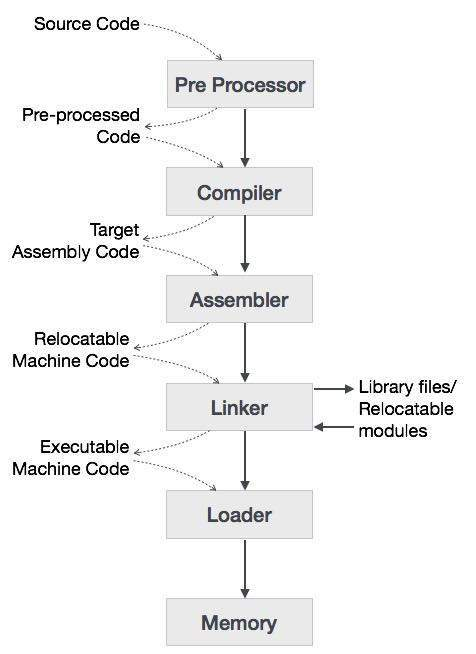
\includegraphics[height=6cm]{img/preprocessor_tricks/language_processing_system.jpg}
    \caption{Language processing system.}
\end{figure}

Let's see the difference in practice. 

\lstinputlisting[language=C,caption={Computing the max (\texttt{src/preprocessor\_tricks/preprocessor\_01.c})}, label={lst:preproc_max}]{src/preprocessor_tricks/preprocessor_01.c}

In Listing \ref{lst:preproc_max}, local variables \texttt{a} and \texttt{b} are mapped to the following stack location in assembly (\texttt{\#} denotes an inline comment):
\begin{verbatim}
mov     DWORD PTR [ebp-12], 0 # a
mov     DWORD PTR [ebp-16], 1 # b
\end{verbatim}
Finding the maximum by calling the macro \texttt{MAX} simply adds more branches to the generated code. The C line below:
\begin{verbatim}
int c = MAX(a, b);
\end{verbatim}
generates the following code:
\begin{verbatim}
    mov     eax, DWORD PTR [ebp-12]
    cmp     eax, DWORD PTR [ebp-16]
    jle     .L6
    mov     eax, DWORD PTR [ebp-12]
    jmp     .L7
.L6:
    mov     eax, DWORD PTR [ebp-16]
.L7:
    mov     DWORD PTR [ebp-20], eax
\end{verbatim}
This is translated into the following pseudocode, where \texttt{[...]} denote memory location:
\begin{verbatim}
    [ebp=12] = 0 # a
    [ebp-16] = 1 # b
    eax = a
    if eax <= b:
        goto .L6
    goto .L7

.L6:
    eax = b
.L7
    [ebp-20] = eax # address ebp-20 stores c
\end{verbatim}
On the other hand, calling the \texttt{max} function:
\begin{verbatim}
int d = max(a, b);
\end{verbatim}
requires pushing the local variables \texttt{a}, \texttt{b} in the stack before the function is called and then popping (\texttt{add esp, 4} pops 4 bytes - one integer) the stack:
\begin{verbatim}
    mov     DWORD PTR [ebp-20], eax
    push    DWORD PTR [ebp-16]
    push    DWORD PTR [ebp-12]
    call    max(int, int)
    add     esp, 8
    mov     DWORD PTR [ebp-24], eax
\end{verbatim}


\subsection{The double evaluation problem of macros}

Passing expressions to macros, such as the output of function, e.g. \texttt{foo()} may hinder the performance of the code due to double evaluation.

\begin{takeaway}[double evaluation problem of macros]
% ref https://stackoverflow.com/questions/39439181/what-is-double-evaluation-and-why-should-it-be-avoided
Passing an expression as an argument to a function-like macro will potentially evaluate that expression twice. That is because the expression will be repeated where ever the macro parameter it takes on, is used in the macro's definition.
\end{takeaway}
This can be remedied by passing values into the macro.

Supposed we have defined a macro for the maximum of two numbers and we want to evaluate py calling two functions:

\begin{lstlisting}[language=c]
#include <stdio.h>

#define MAX(a,b) (((a)>(b))?(a):(b))

int x() { puts("x"); return 0; }
int y() { puts("y"); return 1; }

int main() {
    MAX(x(), y());
}
\end{lstlisting}
\texttt{MAX} in this case will expand to:
\begin{verbatim}
 #define MAX(a,b) ((x() > y()) ? x() : y())   
\end{verbatim}
\begin{verbatim}
When running the C code for \texttt{MAX}, \texttt{x(), y()} are both called once at the test condition and the larger one is called once more. As a result, the program prints:
\begin{verbatim}
x
y
y
\end{verbatim}
Obviously the remedy is to store their returns in local variables and pass the local variables in the macro.

\subsection{Multi-line macros}

Before multi-line are defined, it is important to know about control flow statements not followed by curly braces (``naked'' \texttt{if, else, while, for}).

\begin{takeaway}[naked control flow statements]
A control flow statement that is not followed by {} is considered as a block with the next statement that follows it.
\end{takeaway}

For instance:
\begin{verbatim}
if (condition)
	int a = 1; int b = 2;    
\end{verbatim}
is equivalent to:
\begin{verbatim}
if (condition) {
	int a = 1;
}
int b = 2;    
\end{verbatim}

Back to the main problem -- suppose we want to write a multi-line macro, e.g. a \texttt{FOO} function-like macro that subsequently calls two functions \texttt{foo}, \texttt{bar}. 

\textbf{Attempt 1:}

One naive attempt would be the following:

\lstinputlisting[language=C,caption={First attempt for multi-line macro (\texttt{src/preprocessor\_tricks/preprocessor/preprocessor\_tricks\_02.c})}, label={lst:preproc_foobar1}]{src/preprocessor_tricks/preprocessor_tricks_02.c}

This expends the macro to two statements -- \texttt{foo(42)} and \texttt{bar()} and since ``naked'' \texttt{if} is only followed by one statement, \texttt{bar()} will be executed regardless of the condition.

\textbf{Attempt 2:}

One can try wrapping the two statements in curly braces.
\lstinputlisting[language=C,caption={Third attempt for multi-line macro (\texttt{src/preprocessor\_tricks/preprocessor/preprocessor\_tricks\_03.c})}, label={lst:preproc_foobar2}]{src/preprocessor_tricks/preprocessor_tricks_03.c}

This will be expanded to two statements wrapped in curly braces followed by \texttt{;}:
\begin{verbatim}
if (2 + 2 == 4)
	{ foo(42); bar() };
\end{verbatim}
This in an invalid syntax in C so it will not compile.

\textbf{Attempt 4:}

We can try removing the semicolon after the function-line macro \texttt{FOO2(42)} is called to turn this into a valid \texttt{if} statement:

\lstinputlisting[language=C,caption={Fourth attempt for multi-line macro (\texttt{src/preprocessor\_tricks/preprocessor/preprocessor\_tricks\_04.c})}, label={lst:preproc_foobar2}]{src/preprocessor_tricks/preprocessor_tricks_04.c}

It prints:
\begin{verbatim}
foo
bar
\end{verbatim}
This approach works but it's unconventional as C statements are normally followed by semicolon.

\textbf{Attempt 5:}

One way to consistenly define function-line macros that are followed by a semicolon is by wrapping them in a \texttt{do-while} block as follows:

\lstinputlisting[language=C,caption={Fifth attempt for multi-line macro (\texttt{src/preprocessor\_tricks/preprocessor/preprocessor\_tricks\_05.c})}, label={lst:preproc_foobar5}]{src/preprocessor_tricks/preprocessor_tricks_05.c}

The above program prints the desired output:
\begin{verbatim}
foo
bar
\end{verbatim}
The \texttt{do-while} block ensures the commands inside it will be executed only once. Furthermore, \texttt{do-while} as always followed by a semicolon. Threrefore this idiom not only executes multi-line preprocessor commands, but also must be followed by a semicolon, which makes it consistent with other statements such as function calls. For code maintainability purposes, it's a good practice to wrap \textit{any} macro in \texttt{do-while} -- even single-line ones.
\begin{takeaway}[multi-line macros]
To define a multiple statements \texttt{statement1; statement2; ...} in a macro, they can be wrapped in a \texttt{do-while} block as follows:
\begin{verbatim}
#define FOO(arg1, arg2, ...) do { statement1; statement2; ... } while(0)
\end{verbatim}
\end{takeaway}
\clearpage
%----------------------------- New section ------------------------------%
\section{Integer promotions and signed conversions in C}


\subsection{Mixing floats with ints}

Consider the following program. What will be the output?
\begin{lstlisting}[language=c]
double d = 3.33;
if (d*3 < 10L)
	puts("true");
\end{lstlisting}
Confirming the maths, the output is \texttt{true}, but why? Which value gets converted to which type? Let's look at the main part of the \texttt{clang} disassembly:
\begin{lstlisting}
movsd   xmm0, qword ptr [.LCPI0_0] # xmm0 = double 10
movsd   xmm1, qword ptr [.LCPI0_1] # xmm1 = double 3
movsd   xmm2, qword ptr [.LCPI0_2] # xmm2 = double 3.33
movsd   qword ptr [ebp - 16], xmm2
mulsd   xmm1, qword ptr [ebp - 16] # xmm1 = xmm1 * 3.33
ucomisd xmm0, xmm1
jbe     .LBB0_2 # if 10 below or equal to xmm1 jump to return (.LBB0_2)
<-- omitted -->
call    puts # if xmm0 > xmm1    
\end{lstlisting}
So \texttt{10L} gets converted to double, which makes sense as the other way would make operand \texttt{d*3} lose its precision. A similar conversion occurs in the following snippet too.
\begin{lstlisting}[language=c]
int i = 1;
if (i + 1.5 < i + 2)
	puts("correct!");
\end{lstlisting}
In this case, In this case \texttt{i} gets stored at an \texttt{int} register (e.g. \texttt{eax} register) and when the compiler sees the addition with \texttt{1.5} it copies \texttt{eax} to a floating pointer register (e.g. \texttt{xmm1} and performs the addition with both operands as doubles. The result of \texttt{i+2} also in the end gets stored at a floating point register and the comparison between doubles is made, printing \texttt{correct!}.

According the C ISO \cite{ciso2007}, the following rules apply when an operator operating on \texttt{double} or \texttt{float} and another type \footnote{We don't take into account imaginary numbers for simplicity.}:
\begin{takeaway}[conversion between double/ float and another type -- C ISO 2007, 6.3.1.8/1 ]
\; \\
\begin{enumerate}
    \item First, if the  type of either operand is \texttt{long double}, the other
operand is converted, without change of type domain, to \texttt{long double}.
    \item Otherwise, if the type of either operand is double, the other
operand is converted, without change of type domain, to \texttt{double}.
    \item Otherwise, if the type of either operand is \texttt{float}, the other
operand is converted, without change of type domain, to \texttt{float}. 

To sum up:
\end{enumerate}

\begin{verbatim}
                    long double > double > float > int types
\end{verbatim}
\end{takeaway}


\subsection{Integer sub-types and ranges}

Sometimes integer types and its their sub-types need to be converted from one to another. Such a conversion is called \emphasis{integer promotion}, for example when a \texttt{char} gets converted to \texttt{int}. As a reminder, the table below shows the size of \texttt{int} and its sub-types for most 32-bit machines.

\begin{tabular}{p{0.3\textwidth}p{0.1\textwidth}p{0.15\textwidth}p{0.15\textwidth}p{0.15\textwidth}} \toprule % {|p{4cm}|p{5cm}|}
{Types} & {Bits} & {Naming} & {Min} &{Max} \\ \midrule
    \texttt{char (signed char)} & 8 & byte & $-2^7$ & $2^7-1$\\
    \texttt{unsigned char} &  8 & byte &0 & $2^8-1$\\
    \texttt{short (signed short)} &  16 & word & $-2^{15}$ & $2^{15}-1$\\
    \texttt{unsigned short} &  16 & word & 0 & $2^{16}-1$\\
    \texttt{int (signed int)} &  32 & double word & $-2^{31}$ & $2^{31}-1$\\
    \texttt{unsigned int} &  32 & double word & $0$ & $2^{32}-1$\\
    \bottomrule
\end{tabular}

Note that the sizes in the table are common among many systems but not universal. For example, OpenBSD systems use different numbers of bits. Another integer type, which is \textit{not} a sub-type of \texttt{int} but a super-type of it, is \texttt{long}. It is guaranteed to be at least 32 bits. On Linux Intel architecture, which is used in these notes, its size is the following.

% https://stackoverflow.com/a/271087
\begin{tabular}{p{0.25\textwidth}p{0.15\textwidth}p{0.1\textwidth}p{0.15\textwidth}p{0.1\textwidth}p{0.1\textwidth}} \toprule 
	{Types} & {Architecture} & {Bits} & {Naming} & {Min} &{Max} \\ \midrule
	\texttt{long (signed long)} & Linux IA-32 & 32 & quad word  & $-2^{31}$ & $2^{31}-1$\\
	\texttt{unsigned long} & Linux IA-32 & 32 & quad word & 0 & $2^{32}-1$\\
	\texttt{long (signed long)} & Linux IA/Intel-64 & 64 & quad word & $-2^{63}$ & $2^{63}-1$\\
	\texttt{unsigned long} & Linux IA/Intel-64 & 64 & quad word &0 & $2^{64}-1$\\
    \bottomrule
\end{tabular}


%\url{https://stackoverflow.com/questions/271076/what-is-the-difference-between-an-int-and-a-long-in-c}


\subsection{Integer promotion}

Integer promotion occurs implicitly when we operate on integer sub-types or integers. If an \texttt{int} can represent all values of the original type, the value is converted to an \texttt{int} (and its value is preserved), otherwise it is converted to an \texttt{unsigned int}. Bear in mind integer promotion is not the same as integer conversion, which is studied in another section. The following examples make it clear.

\begin{exmp}[Integer promotion -- signed chars]

Let's take a look at what happens when we operate on integer sub-types together, for example two (signed) \texttt{char} variables.
\begin{lstlisting}[language=c]
char c1 = 100, c2 = 3;
if (c1*c2 > 299)
	puts("Now I know 1st grade maths!");
\end{lstlisting}
The snippet above prints \texttt{Now I know 1st grade maths!}, as it should. But what's the type of \texttt{c1}, \texttt{c2}, \texttt{c1*c2} and \texttt{299} when the comparison is made? The \texttt{gcc} disassembly shows that initially \texttt{c1} and \texttt{c2} are stored in byte (char)-wide local variables but have been copied to 4-byte registers as signed integers\footnote{\texttt{movsx} means move and sign-extend}.  Next, they are multiplied as signed integers (\texttt{imul}) and then the comparison takes place:
\begin{lstlisting}
mov     BYTE PTR [ebp-9], 100
mov     BYTE PTR [ebp-10], 3
movsx   edx, BYTE PTR [ebp-9]
movsx   eax, BYTE PTR [ebp-10]
imul    eax, edx
cmp     eax, 299
\end{lstlisting}
\qedblack
\end{exmp}

\begin{exmp}[Integer promotion -- signed char and unsigned char]
We introduce a subtle change to the previous example, defining one \texttt{signed char} and one \texttt{unsigned char} instead, so the snippet looks like:
\begin{lstlisting}[language=c]
char c1 = 100;
unsigned char c2 = 3;
if (c1*c2 > 299)
	puts("Now I know 1st grade maths!");
\end{lstlisting}
Then \texttt{c1} is zero-extended when copied to a 4-byte general register to store local variable \texttt{c2} as unsigned but the final result, i.e. \texttt{c1*c2} is treated as a \texttt{signed int}, as indicated by the \texttt{imul}:
\begin{lstlisting}
movsx   eax, byte ptr [ebp - 5]
movzx   ecx, byte ptr [ebp - 6]
imul    eax, ecx
\end{lstlisting}
The compiler would prefer to represent expression \texttt{c1*c2} as \texttt{signed int} even if both \texttt{c1,c2} were defined \texttt{unsigned char}! \qedblack
\end{exmp}

\begin{exmp}[Integer promotion -- unsigned char and unsigned char]
In this case, have define \texttt{c1} and \texttt{c2} as \texttt{unsigned char}. However, we assign -6 to one of them. What gets printed?
\begin{lstlisting}[language=c]
unsigned char c1 = 100;
unsigned char c2 = -6;
printf("%d\n", c1*c2);
\end{lstlisting}
The \texttt{gcc} disassembly sheds some light.
\begin{lstlisting}
mov    BYTE PTR [ebp-0xa],0x64
mov    BYTE PTR [ebp-0x9],0xfa
movzx  edx,BYTE PTR [ebp-0xa]
movzx  eax,BYTE PTR [ebp-0x9]
imul   eax,edx
\end{lstlisting}
So what actually gets stored in \texttt{c2} (local variable \texttt{[ebp-0x9]}) is \texttt{0xfa = 250}, therefore the compiler mapped -6 to the \texttt{unsigned char} range  $[0, 255]$\footnote{When mapping from one range of equal width to another, the byte representation doesn't change, only the way we interpret the bytes does.}, doing what the type of \texttt{c2} defined. Although \texttt{c1} and \texttt{c2} are correctly represented by unsigned values (\texttt{movzx} instruction), the expression \texttt{c1*c2} is once again treated as signed integer, as indicated by \texttt{imul}. \qedblack

We've seen what happens when operations between \texttt{int} sub-types are performed. But what if two (signed) \texttt{int}s are operated and the result is not small enough to fit in the \texttt{signed int} range?
\begin{exmp}[When result doesn't fit in \texttt{signed int}.]

\marginnote{In C, integers are signed by default.}In this example, we have the maximum integer than can be represented by the 32-bit range, i.e. $2^{31}-1$. We want to double it and compare it to zero, which should of course be true. But we want the operation to be performed between unsigned integers, as signed cannot represent the result. If we simply compared:
\begin{lstlisting}[language=c]
2*i > 0
\end{lstlisting}
, then 2, \texttt{i}, 0 are all signed and we'd end up comparing -2 to 0. The way to make the compiler understand that the result should be performed in \texttt{unsigned} if it doesn't fit in \texttt{signed} would be to make at least of the operands unsigned, e.g. as follows: 
\begin{lstlisting}[language=c]
#include <stdio.h>
#include <limits.h>

void main(int argc, char *argv[])
{
	signed int i = INT_MAX; // 2^31 - 1 for 32b systems
	if (2U*i > 0)
		printf("correct! unsigned result = %u" , 2U*i);
}
\end{lstlisting}
\end{exmp}
Then
\begin{verbatim}
correct! unsigned result = 4294967294   
\end{verbatim}
is printed (i.e. $2^{32}-2$, or \texttt{0xfffffffe}), as it should. As a final note, notice again that the expression \texttt{2*i > 0} operates on \texttt{unsigned int} if either of \texttt{2} (e.g. \texttt{2U}), \texttt{i}, or \texttt{0} is unsigned (\texttt{0U}). The next section explains such conversions.\qedblack
\end{exmp}
\marginnote{Integer promotions occur every time we operate with integer sub-types.}The last 4 examples can be justified by the following C ISO standard \cite{ciso2007}.
\begin{takeaway}[integer promotion definition -- C ISO 2007, 6.3.1.1/2]
If an \textup{\texttt{int}} can represent all values of the original type or \textup{\texttt{int}} sub-type, the value is converted to an \textup{\texttt{int}}; otherwise, it is converted to an \textup{\texttt{unsigned int}}. These are called \emphasis{integer promotions}. All other types are unchanged by integer promotions. 
\end{takeaway}




\subsection{IEEE priority (rank) rules}


When operating on both signed and unsigned, there are a few things that C takes into account to determine the result, in order of priority:
\begin{enumerate}
    \item The width of each type (e.g. 256 for \texttt{signed char} and \texttt{unsigned char} etc. The width of each type can be mapped to the ``rank'' in the C ISO. Integer rank defines which type will be converted to what.
    \item Whether the operands are signed or unsigned, and whether they're different or not.
\end{enumerate}
Regarding the rank, the ISO\cite{ciso2007} defines the following:
\begin{takeaway}[integer rank -- C ISO 2007 6.3.1.1/2]
\begin{lstlisting}
rank(long long) > rank(long) > rank(int) > rank(short) > rank(char)
\end{lstlisting}
The rank of any unsigned integer type shall equal the rank of the corresponding
signed integer type, if any. Rank is essentially the width a type can represent.
\end{takeaway}

Here are some typical cases. Try to guess what rules apply given the rank and the signedness. Following the examples, the rule from C ISO is quoted. 

\begin{exmp}[Mixing smaller int sub-type with larger sub-type]
\begin{lstlisting}[language=c]
signed char sc = -1;
unsigned short ush = 0;
(sc + ush < ush)? puts("-1 < 0"): puts("-1 >= 0");
\end{lstlisting}
In this case, we operate on \texttt{int} sub-types \texttt{signed char} and \texttt{unsigned short}. First, \texttt{+} takes place. According to the promotions, \texttt{sc} and \texttt{ush} are both promoted to \texttt{int} before the addition, both obtaining the same rank and yielding \texttt{-1}. So we compare the latter result to \texttt{ush}, which is zero. \texttt{ush} is also promoted to \texttt{int} before the comparison, resulting in the condition printing  \texttt{-1 < 0}. \qedblack
\end{exmp}


\begin{exmp}[Mixing int sub-type with signed int]
This is similar to the previous, except \texttt{si} does not have to be promoted to \texttt{int} as it already is -- only \texttt{ssh} will, maintaining its value.
\begin{lstlisting}[language=c]
signed short ssh = -1;
int si = 0;
(ssh + si < si)? puts("-1 < 0"): puts("-1 >= 0");
\end{lstlisting}
The result is \texttt{-1 < 0}.
\end{exmp}


\begin{exmp}[mixing signed int with unsigned int]

We have the same code with the previous example, except now we compare \texttt{ssh + si} to unsigned zero (\texttt{0U}).
\begin{lstlisting}[language=c]
signed short ssh = -1;
int si = 0;
(ssh + si < 0U)? puts("-1 < 0"): puts("-1 >= 0");
\end{lstlisting}
The result is \texttt{-1 > 0} so \texttt{ssh + si} must have been converted to \texttt{unsigned int}. Indeed, \texttt{printf("\\n\%u\\n", ssh + si)} gives 4294967295, which is $2^{32}-1$, which is the upper limit of \texttt{unsigned int} for 32-bit systems. To summarise, the bottom to top order is:
\begin{verbatim}
ssh => int
(ssh + si) => int
(ssh + si < 0U) => ssh + si => unsigned int
\end{verbatim}
It seems that if we have operate on two types with the same rank and different sign, the compiler prefers to convert \texttt{signed} to \texttt{unsigned}. \qedblack
\end{exmp}


\begin{exmp}[Mixing long with int]
Now we have two types with different rank -- \texttt{unsigned long} and \texttt{int}. 
\begin{lstlisting}[language=c]
int si = -1;
unsigned long ul = 0;
(si + ul < ul)? puts("[4]: -1 < 0"): puts("[4]: -1 >= 0");
\end{lstlisting}
On a 32-bit system, \texttt{unsigned long} and \texttt{int} have the same width of 4 bytes therefore the same rank, therefore the output would depend on signedness; we've seen that signed is preferred to be converted to unsigned when the rank is the same so the result is \texttt{-1 >= 0}.

On a 64-bit system, the result would also be \texttt{-1 <= 0}. The rank of \texttt{unsigned long} is same the rank of \texttt{long} and is greater than the rank of \texttt{int}. So \texttt{si} would be converted to \texttt{unsigned long} etc.

The disassembly shows how the comparison is implemented in the generated code. The relevant parts are the following, and especially the \texttt{jbe} instruction.
\begin{lstlisting}
mov DWORD PTR [rbp-0xc],0xffffffff ; int si = -1
mov QWORD PTR [rbp-0x8],0x0        ; unsigned long ul = 0
mov eax,DWORD PTR [rbp-0xc]
movsxd rdx,eax                     ; eax = 0xffffffffffffffff
mov rax,QWORD PTR [rbp-0x8]        ; rax = ul = 0
add rax,rdx                        ; rax += si
cmp QWORD PTR [rbp-0x8],rax
jbe 0x1178 <main+63>               ; if (PTR[rbp-0x8] <= rax)...
\end{lstlisting}
\end{exmp}
The instruction \texttt{jbe} treats the comparison operands as unsigned.

On the other hand, consider defining \texttt{ul} as \texttt{long}. Then \texttt{si} wouldn't have to be converted to \texttt{unsigned long} (in fact not even to long as it's simply compared to zero, hence the \texttt{DWORD}!). We'd end up with:
\begin{lstlisting}
mov DWORD PTR [rbp-0xc],0xffffffff
cmp DWORD PTR [rbp-0xc],0x0
jns 0x116b <main+50>
\end{lstlisting}
\texttt{cmp} compares \texttt{si} to zero. \texttt{jns} (Jump if Not Sign) checks its sign, i.e. its first bit, and branches accordingly. \qedblack

\begin{exmp}[signed char to unsigned char] 
\begin{lstlisting}
char sc = -2;
unsigned char uc = 1;
(sc + uc == -1)? puts("[5] -1"): puts("[5] != -1");
\end{lstlisting}
In this case, both \texttt{sc} and \texttt{uc} are promoted to integer before the addition and the sign and values are preserved:
\begin{lstlisting}
movsx  edx,BYTE PTR [rbp-0x2]
movsx  eax,BYTE PTR [rbp-0x1]
add    eax,edx
cmp    eax,0xffffffff
jne    0x117d <main+52>
\end{lstlisting}
\texttt{[5] -1} is printed. The result would also be true in the following cases:
\begin{lstlisting}[language=c]
(sc + uc == -1U)
(sc + uc == UINT_MAX)
(sc + uc == 0xffffffff)
\end{lstlisting}
\qedblack
\end{exmp}

\begin{exmp}[signed int to unsigned int]
signed int si = -5;
unsigned int ui = 2;
(si + ui == -3)? puts("[6]: -5+2==-3"): puts("[6]: -5+2!=-3");
In this case, \texttt{si} and \texttt{ui} have the same rank but different sign. Because \texttt{int} can represent both, no conversion is necessary therefore \texttt{[6]: -5+2==-3} is printed.
\qedblack
\end{exmp}

The code for all examples is found in \texttt{src/int\_conv/conversions.c}. The following C ISO extract applies to the above examples. Note that when we operate on signed and unsigned it is \textit{not always} the case that signed will be converted to unsigned (paragraph 4).
\begin{takeaway}[C ISO 2007 -- 6.3.1.8/1]
\; \\
\begin{enumerate}

\item If both operands have the same type, then no further conversion is needed. 

\item Otherwise, if both operands have signed integer types or both have unsigned integer  types,  the  operand  with  the  type  of  lesser  integer  conversion  rank  is converted to the type of the operand with greater rank.

\item Otherwise,  if  the  operand  that  has  unsigned  integer  type  has  rank  greater  or equal  to  the  rank  of  the  type  of  the  other  operand,  then  the  operand  with signed  integer  type  is  converted  to  the  type  of  the  operand  with  unsigned integer type.

\item Otherwise, if the type of the operand with signed integer type can represent all of the values of the type of the operand with unsigned integer type, then the  operand  with  unsigned  integer  type  is  converted  to  the  type  of  the operand with signed integer type.

\item Otherwise,   both   operands   are   converted   to   the   unsigned   integer   type corresponding to the type of the operand with signed integer type.
\end{enumerate}
\end{takeaway}
Finally, if it's not clear yet, to convert a negative signed to unsigned we do the following:

\begin{verbatim}
while (number < 0) {
    number += MAX_UNSIGNED_INT + 1
}
\end{verbatim}
This does not change the binary representation of the number -- only the way it's interpreted. In binary, negative numbers are represented by \emphasis{2's complement}. For example, on a 4-bit machine, we have the signed
\begin{verbatim}
-2 = 1110b
\end{verbatim}
Adding \texttt{MAX\_UNSIGNED\_INT = 16} does not change the bits of the number. Using the magnitude representation instead of 2's complement, we have
\begin{verbatim}
-2 + MAX_UNSIGNED_INT = 14 = 1110b
\end{verbatim}

These are were basics of how integers are handled by the compiler in C.


% https://www.oreilly.com/library/view/c-in-a/0596006977/ch04.html
% https://aticleworld.com/signed-and-unsigned-integers/
% https://github.com/LambdaSchool/CS-Wiki/wiki/Casting-Signed-to-Unsigned-in-C 
% https://embeddedgurus.com/stack-overflow/2009/08/a-tutorial-on-signed-and-unsigned-integers/
% https://aticleworld.com/signed-and-unsigned-integers/
% https://github.com/LambdaSchool/CS-Wiki/wiki/Casting-Signed-to-Unsigned-in-C
% https://embeddedgurus.com/stack-overflow/2009/08/a-tutorial-on-signed-and-unsigned-integers/
% http://www.idryman.org/blog/2012/11/21/integer-promotion/
% https://stackoverflow.com/questions/17312545/type-conversion-unsigned-to-signed-int-char/17312930#17312930
% http://www.idryman.org/blog/2012/11/21/integer-promotion/
% https://pleasestopnamingvulnerabilities.com/integers.html



% https://www.cs.virginia.edu/~evans/cs216/guides/x86.html
% Redefining IMUL and IDIV Are you still reading these subtitles?

\clearpage
\input{chapters/inline.tex}
\clearpage
\input{chapters/operators.tex}
\clearpage
%------------------------------ New section ------------------------------%
\section{Advanced pointer usages}

\subsection{Const pointer vs pointer to const}
%https://stackoverflow.com/questions/21476869/constant-pointer-vs-pointer-to-constant
In C, we often want to make a pointer point to a constant address or reference a constant. The syntax for both of these instruction is similar but there is a subtle difference. In this section, shed some light on this syntax difference to make it easy to remember.

\subsubsection{Constant pointer}

The syntax for constant point (constant address) is as follows:
\begin{verbatim}
int*    const    ptr;
\end{verbatim}
This is expression is read right from left. Let's read it step-by-step.
\begin{minted}{C}
    int*    const    ptr;
//                   ~~~~  
//                   Define a pointer ptr
//          ~~~~~
//          that is constant
//  ~~~~
//  and points to an integer variable
\end{minted}
Therefore defines a constant point (the address it points to cannot change) to data of type \texttt{int}. Attempting to change the address results in a complication error. A toy example is listed below.
\lstinputlisting[language=C,caption={DOs and DONTs of constant pointer (\texttt{src/pointers/const\_ptr.c})}, label={lst:const_ptr_code}]{src/pointers/const_ptr.c}
It prints \texttt{3}.



\subsubsection{Pointer to constant}
The following pointer cannot have its value changed.
\begin{minted}{C}
    const    int    *ptr;
//                  ~~~~ 
//                  Define a pointer ptr
//           ~~~
//           that points to int data
//  ~~~~~
//  which data are constant
\end{minted}
It's clear that the \texttt{const} specifier acts upon the value (\texttt{int}), therefore the pointer is of constant value (pointer to \texttt{const}). Attempting to dereference the pointer and change its value results in a compilation error. However, we can still change the data it points to. A toy example is also listed below.
\lstinputlisting[language=C,caption={DOs and DONTs of pointer to const (\texttt{src/pointers/ptr\_to\_const.c})}, label={lst:ptr_to_const_code}]{src/pointers/ptr_to_const.c}
The example code prints \texttt{2}.


%=-=-=-=-=-=-=-=-=-=-=-=-=-=-=-=-=-=-=-=-=-=-=-=-=-=-=-=-=-=-=-=-=-=-=-=-=-=-=-=-
% References
%=-=-=-=-=-=-=-=-=-=-=-=-=-=-=-=-=-=-=-=-=-=-=-=-=-=-=-=-=-=-=-=-=-=-=-=-=-=-=-=-
\newpage
\printbibliography


%=-=-=-=-=-=-=-=-=-=-=-=-=-=-=-=-=-=-=-=-=-=-=-=-=-=-=-=-=-=-=-=-=-=-=-=-=-=-=-=-
% Appendices
%=-=-=-=-=-=-=-=-=-=-=-=-=-=-=-=-=-=-=-=-=-=-=-=-=-=-=-=-=-=-=-=-=-=-=-=-=-=-=-=-
\newpage
\appendix

\section{Appendices}


% ------------------------ New appendix ------------------------ %
\newpage
\subsection{ANSI C vs GNU C}
\label{app:gnu_vs_iso}
In the main text, we have used the terms ``ISO C, ANSI C'' and ``GNU C''. They mean different things.

\begin{itemize}
    % https://stackoverflow.com/questions/17206568/what-is-the-difference-between-c-c99-ansi-c-and-gnu-c
    \item GNU C: GNU is a unix like operating system (www.gnu.org) \& somewhere GNU's project needs C programming language based on ANSI C standard. GNU use GCC (GNU Compiler Collection) compiler to compile the code. It has C library function which defines system calls such as malloc, calloc, exit...etc
    % https://www.linuxquestions.org/questions/programming-9/gnu-c-and-ansi-c-520509/
    \item ANSI C is a standardised version of the C language. As with all such standards it was intended to promote compatibility between different compilers which tended to treat some things a little differently.
    \item standard specified in the ANSI X3.159-1989 document became known as ANSI C, but it was soon superseded as it was adopted as an international standard, ISO/IEC 9899:1990.
\end{itemize}




% ------------------------ New appendix ------------------------ %
\newpage
\subsection{\texttt{idiv} and \texttt{imul} instructions}
\label{app:idiv_imul}
\texttt{imul} and \texttt{idiv} instructions are used in assembly to perform multiplication or division with signed integers. \texttt{mul} and \texttt{div} are their respective unsigned instructions. We'll be using Intel IA-32 instructions for convenience. 


\subsubsection{\texttt{imul}}
 

% ref http://www.godevtool.com/TestbugHelp/UseofIMUL.htm
The IMUL instruction takes one, two or three operands. It can be used for byte, word or dword operation. IMUL only works with signed numbers. The result is the correct sign to suit the signs of the multiplicand and the multiplier, therefore the if necessary (e.g. negative) is \textit{sign extended} following the 2's complement rules. The size of the result maybe up to twice of the input size. Therefore when using a user-specified register as the destination (table below), the result is truncated to the register size and it's up to the user to prevent information loss. For 32-bit architectures, the result may be represented with up to 64 bits. Finally, remember that 
\begin{itemize}
    \item 32-bit signed range represents numbers $[-2^{31},2^{31}-1]$,
    \item 32-bit unsigned range represents numbers $[0, 2^{32}-1]$.
\end{itemize}


\lstinputlisting[caption={\texttt{imul} simple demonstration. (\detokenize{src/imul_only.asm)}.}]{src/imul_only.asm}

Note that when the result in EDX:EAX is negative, the whole double register is sign extended, to 64 bits, e.g. when we obtain -20, EDX:EAX stores \texttt{0xffffffff:0xffffffec}.


% 86 intel: https://www.felixcloutier.com/x86/imul
\begin{tabular}{p{0.25\textwidth}p{0.37\textwidth}p{0.3\textwidth}} \toprule % {|p{4cm}|p{5cm}|}
{Syntax} & {Description} & {Types} \\ \midrule
    \texttt{imul src} & {\texttt{EDX:EAX = EAX * src}} & {\texttt{src: r/m32}} \\
    
    \texttt{imul dst, src} & {\texttt{dst = src * dst}} & {\texttt{dst: r32}, \texttt{src:r32/m32}}\\
    \texttt{imul dst, src1, src2} & {\texttt{dst = src1 * src2}} & {\texttt{dst: r32},
    \texttt{src1: r32/m32}, \texttt{src2: val32}} \\ \bottomrule
\end{tabular}


% ------------------------ New appendix ------------------------ %
\subsubsection{\texttt{idiv}}
% ref Redefining IMUL and IDIV Are you still reading these subtitles?

% see https://www.felixcloutier.com/x86/idiv
% https://www.aldeid.com/wiki/X86-assembly/Instructions/idiv
Assuming 32-bit architecture, \texttt{idiv src} performs signed division. It divides the 64-bit register pair  \texttt{edx:eax} registers by the source operand \texttt{src} (divisor). It  and stores the result in the the pair \texttt{edx:eax}. It stores the quotient in \texttt{eax} and the remainder in \texttt{edx}. Non-integral results are truncated (chopped) towards 0.
\begin{tabular}{p{0.25\textwidth}p{0.37\textwidth}p{0.3\textwidth}} \toprule % {|p{4cm}|p{5cm}|}
{Syntax} & {Description} & {Types} \\ \midrule
    \texttt{idiv src} & {\texttt{EDX = EDX:EAX \% src},\quad\quad\quad\quad\quad\quad\quad \texttt{EAX = EDX:EAX / src}} & {\texttt{src: r/m32}} \\
    \bottomrule
\end{tabular}

However, we need to be careful before using \texttt{idiv}. Check out the following example.

At line 18, \texttt{edx = 0x20 = 32}. We pollute \texttt{eax} with \texttt{eax = 11 = 0xb} and want to divide by \texttt{ebx = 2}  so the program will try to divide \texttt{edx:eax = 0x200000000b} by \texttt{2} and store the quotient \texttt{0x200000000b/2 = 68719476741} in \texttt{eax}. \marginnote{Always make sure that \texttt{eax} is zero before \texttt{idiv} (or \texttt{div}).}However, $68719476741 > 2^{32}$ so it cannot fit -- the program will receive a \texttt{SIGFPE} (arithmetic exception) signal by the kernel and exit.

% also  https://stackoverflow.com/questions/38416593/why-should-edx-be-0-before-using-the-div-instruction/38416896
\lstinputlisting[caption={\texttt{idiv} demonstration for unsigned division. (\detokenize{src/idiv_wrong1.asm)}.}]{src/idiv_wrong1.asm}


%%%%%%%%%%%%%
% negative idiv
%
% https://stackoverflow.com/questions/27385132/divide-a-negative-with-a-positive
% https://stackoverflow.com/questions/54000965/what-is-signed-divisionidiv-instruction
Let's examine what happens when we divide \texttt{EDX:EAX} by a negative number. 

\lstinputlisting[caption={\texttt{idiv} demonstration for signed division. (\detokenize{src/idiv_wrong2.asm)}.}]{src/idiv_wrong2.asm}

In the first example, we attempt to divide $-21$ by $2$ so we move $-21$ to \texttt{eax}, which is represented in hex as \texttt{eax = 0xffffffeb}. \texttt{edx} is zero so \texttt{idiv} will try to define the positive number (leading 0) in \texttt{edx:eax = 00000000:ffffffeb = 4294967275}. As a result, $4294967275$ will be divided by 2, writing \texttt{4294967275 div 2} = \texttt{2147483637} to \texttt{eax} and \texttt{4294967275 mod 2 = 1} to \texttt{edx}.

To get the value right, we need to ensure the whole divident (\texttt{edx:eax}) is negative. This is done by sign extending \texttt{edx} into \texttt{eax}, i.e. set \texttt{edx = 0xffffffff} is \texttt{eax < 0}. Example 2 correctly performs the division, writing \texttt{0xffffffff} (-1) to \texttt{edx} and \texttt{0xfffffff6} (-10) to \texttt{eax}. 

The next section describes an instruction that can generalise this zero/sign extension before \texttt{idiv}.


% ------------------------ New appendix ------------------------ %
\subsubsection{The \texttt{cdq} instruction}

% see https://stackoverflow.com/a/25489305
\texttt{cdq} converts the doubleword (32 bits) in \texttt{EAX} into a quadword in \texttt{EDX:EAX} by sign-extending \texttt{EAX}  into \texttt{EDX} (i.e. each bit of EDX is filled with the most significant bit of EAX). 

For example, if \texttt{EAX}  contained \texttt{0x7FFFFFFF} we'd get 0 in \texttt{EDX}, since the most significant bit of \texttt{EAX} is clear. But if we had \texttt{EAX = 0x80000000} we'd get \texttt{EDX = 0xFFFFFFFF} since the most significant bit of \texttt{EAX} is set. The point of \texttt{cdq} is to set up \texttt{EDX} prior to a division by a 32-bit operand, since the dividend is \texttt{EDX:EAX}. 

The program below demonstrates the instruction.

\lstinputlisting[caption={Chaining \texttt{cdg} with \texttt{idiv} to avoid potential arithmetic errors due to sign. (\detokenize{src/idiv_correct.asm)}.}]{src/idiv_correct.asm}

After line 16, \texttt{edx = 0x2} and \texttt{eax = 0x5}. After line 21, \texttt{edx = 0xffffffff} and \texttt{eax = 0xffffffea}. After line 22, \texttt{edx = 0xfffffffe = -2} and \texttt{eax = 0xffffffbf = -5}.


% ------------------------ New appendix ------------------------ %
\newpage
\subsection{Increment and decrement operators}
\label{app:pre_post_increment}

\subsubsection{Pre vs post increment operator}
%\label{app:my_cool_appendix}

In C, pre-increment (\texttt{++i}) and post-increment (\texttt{i++}) work slightly differently. Pre-decrement (\texttt{--i}) and post-decrement (\texttt{i--}) also work in a similar manner. Pre-increment means that the variable is incremented and the incremented value is returned. Post-increment means that the variable is returned as its original value and then incremented. The way to remember them is:
\begin{itemize}
    \item \textit{pre}$\rightarrow$ \textit{first} increment, then evaluate, 
    \item \textit{post}$\rightarrow$ increment \textit{after} evaluating.
\end{itemize}
The following table summarises the differences. In the equivalent assembly code, we can see that
\begin{itemize}
    \item in the first case (\texttt{j=i++}), \texttt{eax} register stores the initial value of local variable \texttt{i=0x42}. Next, \texttt{edx=eax+1=0x43}. Finally, \texttt{edx} is copied to \texttt{i} and \texttt{eax} is coped to \texttt{j} so \texttt{i=0x43, j=0x42}.
    \item In the second case (\texttt{j=++i}), \texttt{eax} stores again \texttt{i=0x42}. \texttt{eax} gets incremented. Then, it gets copied to both local variables \texttt{i} and \texttt{j} so \texttt{i=0x42, j=0x42}.
\end{itemize}


\begin{table}[ht]
\centering
% To place a caption above a table
\caption{Post vs pre-increment differences and generated code.}
\begin{tabular}{ccccc} \toprule
    Operation & How it appears & Pseudocode & \begin{tabular}{@{}c@{}}Assembly code  \footnote{Instruction \texttt{lea edx, [eax+0x1]} achieves the same as incrementing \texttt{eax} and moving it to \texttt{edx}.} \\ (initially \texttt{\textcolor{magenta!60!black}{i}=0x42, \textcolor{cyan!40!black}{j}=0x41})\end{tabular} & \begin{tabular}{@{}c@{}}Final\footnote{\texttt{j} of course doesn't need to be initialised but it was added just for clarity in the disassembly.} values  \\ (initially \texttt{i=0x42})\end{tabular}  \\ \midrule
    
    Post-increment &
    \texttt{j=i++} &
    \begin{tabular}{@{}c@{}}\texttt{j=i} \\ \texttt{i++}\end{tabular} & \begin{tabular}{@{}l@{}l@{}l@{}l@{}l@{}}
    \texttt{mov    \textcolor{magenta!60!black}{DWORD PTR [ebp-0x10]},0x42} \\
    \texttt{mov    \textcolor{cyan!40!black}{DWORD PTR [ebp-0xc]},0x41} \\
    \texttt{mov    eax,\textcolor{magenta!60!black}{DWORD PTR [ebp-0x10]}} \\
    \texttt{lea    edx,[eax+0x1]} \\
    \texttt{mov    \textcolor{magenta!60!black}{DWORD PTR [ebp-0x10]},edx} \\
    \texttt{mov    \textcolor{cyan!40!black}{DWORD PTR [ebp-0xc]},eax} \end{tabular} &
    \texttt{i=0x43, j=0x42}
    \\
    
    \rule{0pt}{4ex} & \rule{0pt}{4ex}  & \rule{0pt}{4ex}  & \rule{0pt}{4ex}  \\   
    
    Pre-increment & \texttt{j=++i} & \begin{tabular}{@{}c@{}}\texttt{i++} \\ \texttt{j=i}\end{tabular} &  
    \begin{tabular}{@{}l@{}l@{}l@{}l@{}l@{}}
    \texttt{mov    \textcolor{magenta!60!black}{DWORD PTR [ebp-0x10]},0x42} \\
    \texttt{mov    \textcolor{cyan!40!black}{DWORD PTR [ebp-0xc]},0x41} \\
    \texttt{mov    eax,\textcolor{magenta!60!black}{DWORD PTR [ebp-0x10]}} \\
    \texttt{add    eax,0x1} \\
    \texttt{mov    \textcolor{magenta!60!black}{DWORD PTR [ebp-0x10]},eax} \\
    \texttt{mov    \textcolor{cyan!40!black}{DWORD PTR [ebp-0xc]},eax}
    \end{tabular} &
    \texttt{i=0x43, j=0x43}
    \\ \bottomrule
\end{tabular}
\end{table}

\begin{exmp}
In the following snippet, pre (post) increment evaluate before (after) the array indexing. Notice how the increment operator writes to its ``lvalue'' (either index \texttt{i} or array \texttt{arr}) each time.


\begin{lstlisting}[language=c]
#include <stdio.h>

#define SIZE 5

int main(int argc, char *argv[])
{
	int arr[SIZE] = {0, 1, 2, 4, 5};
	int i = 0;

	printf("%d, ", arr[i++]);
	printf("%d, ", arr[i]);
	printf("%d, ", arr[++i]);
	printf("%d, ", arr[i]++);
	printf("%d\n", ++arr[i]);
	for (i = 0; i < SIZE; ++i) 
		printf("arr[%i] = %d, ", i, arr[i]);
	printf("\n");

	return 0;
}
\end{lstlisting}
The output is:
\begin{verbatim}
0, 1, 2, 2, 4
arr[0] = 0, arr[1] = 1, arr[2] = 4, arr[3] = 4, arr[4] = 5, 
\end{verbatim}

\end{exmp}


\subsubsection{How much does the \texttt{++} increase the value?}

When we have an integers, increment operator increases the value by one. For floats/ doubles it also works the same. What if we have a pointer that points to some address and increment its value? 

Assume we have an array of \texttt{int} called \texttt{arr} and a pointer \texttt{p\_arr} pointing to its first element. Assume  an \texttt{int} takes 4 bytes. Then it would be natural to want to move from \texttt{arr[0]} to \texttt{arr[1]}, which are 4 bytes away. So incrementing the pointer would make sense only if it was incremented by 4 (bytes). In general, here's what happens when we increment a pointer of type T. \todo{figure for explanation}
\begin{takeaway}
% ref https://stackoverflow.com/questions/5610298/why-does-int-pointer-increment-by-4-rather-than-1
When we increment a \texttt{T*}, it moves \texttt{sizeof(T)} bytes. It doesn't make sense to move any other value as then the pointer would point to incomplete data.
\end{takeaway}
The following example confirms it.
\begin{exmp}
\begin{lstlisting}[language=c]
#include <stdio.h>

#define SIZE 5

int main(int argc, char *argv[])
{
	int arr[SIZE] = {0, 1, 2, 3, 4};
	short int sarr[SIZE] = {0, 1, 2, 3, 4};
	int* p_arr = &arr[0]; // point to beginning - same as p_arr = arr 
	short int* p_sarr = &sarr[0];

	printf("p_arr points to: 0x%x\n", p_arr);
	printf("next, p_arr points to: 0x%x\n", ++p_arr);
	printf("p_arr contains: %d\n", *p_arr);

	printf("p_sarr points to: 0x%x\n", p_sarr);
	printf("next, p_sarr points to: 0x%x\n", ++p_sarr);
	printf("p_sarr contains: %d\n", *p_sarr);

	return 0;
}
\end{lstlisting}
\end{exmp}
The output is:
\begin{verbatim}
p_arr points to: 0xbfc8ce78
next, p_arr points to: 0xbfc8ce7c
p_arr contains: 1
p_sarr points to: 0xbfc8ce6e
next, p_sarr points to: 0xbfc8ce70
p_sarr contains: 1
\end{verbatim}
In this system, \texttt{int} takes 4 bytes and \texttt{short int} 2. Hence we move from \texttt{0xbfc8ce78} to \texttt{0xbfc8ce78+4} in the first case and from \texttt{0xbfc8ce6e} to \texttt{0xbfc8ce6e+2} in the second.



% ------------------------ New appendix ------------------------ %
\newpage
\subsection{Find the number of elements in array}

\url{https://stackoverflow.com/questions/27518251/how-does-sizeof-know-the-size-of-array}\\
\url{https://stackoverflow.com/questions/671790/how-does-sizeofarray-work}\\


\end{document}.
